%%%%%%%%%%%%%%%%%%%%%%%%%%%%%%%%%%%%%%%%%%%%%%%%%%%%%%%%%%%%%%%%%%%%%%%%%%%%%%%
% CHAPTER 15: WILLINGNESS TO EFFECTIVELY CHANGE (WEC)
% Frage 7: Wie gross ist die Willingness to Effectively Change 
%          im Moment of Truth along the Behavioral Change Journey?
%%%%%%%%%%%%%%%%%%%%%%%%%%%%%%%%%%%%%%%%%%%%%%%%%%%%%%%%%%%%%%%%%%%%%%%%%%%%%%%

\chapter{Willingness to Effectively Change: The Moment of Truth}
\label{ch:wec}

%------------------------------------------------------------------------------
% DIE 9 FRAGEN NAVIGATION BOX
%------------------------------------------------------------------------------
\BCMQuestionNav{15}

%------------------------------------------------------------------------------
% CORE FRAMEWORK INTEGRATION BOX
%------------------------------------------------------------------------------
\begin{tcolorbox}[colback=purple!5!white, colframe=purple!75!black,
    title=\textbf{10C CORE Framework Integration}]
\textbf{This chapter synthesizes:}
\begin{itemize}[nosep]
    \item \textbf{CORE-AWARE (AU):} Awareness function $A(\cdot)$ transforms $U_{pot} \to U_{eff}$
    \item \textbf{CORE-READY (AV):} Willingness function $WAX \geq \theta$ determines action
    \item \textbf{CORE-STAGE (AW):} BCJ phase $\varphi \in \{1,...,5\}$ locates agent in journey
    \item \textbf{CORE-WHAT (C):} Utility dimensions (INU/KNU/IDN × FEPSDE)
    \item \textbf{CORE-WHEN (V):} Context modulation via $\Psi$-dimensions
\end{itemize}

\textbf{Key equation:} $Action \Leftrightarrow WAX \geq \theta$ where WAX = Willingness to Act
(see Appendix~\ref{app:core-ready} for 99+ axioms specifying $WAX$ dynamics)
\end{tcolorbox}

%------------------------------------------------------------------------------
% METHODOLOGICAL NOTE: EXCLUSION PRINCIPLE
%------------------------------------------------------------------------------
\begin{tcolorbox}[colback=red!5!white, colframe=red!75!black,
    title=\textbf{Methodological Note: The Exclusion Principle (Appendix FRM)}]
\textbf{Following Appendix FRM (LIT-FEHR-METHOD):}

This chapter combines multiple CORE components. Following the \textbf{Exclusion Principle}:
\begin{itemize}[nosep]
    \item \textbf{Null Hypothesis:} Components interact additively ($\gamma = 0$)
    \item \textbf{Alternative:} Non-additive interactions exist ($\gamma \neq 0$)
    \item \textbf{Scientific Value:} WEC gains value where it shows interactions that additive models miss
\end{itemize}

\textbf{Practical implication:}
\begin{itemize}[nosep]
    \item Test whether $WEC = WAX + BCJ + BCS$ (additive) works first
    \item Only claim $WEC = f(WAX \times BCJ \times BCS)$ (multiplicative) if additive fails
    \item Each interaction claim ($\alpha_{BCJ}$, $\beta_{BCS}$) must be empirically justified
\end{itemize}
\end{tcolorbox}

%------------------------------------------------------------------------------
\section{Introduction: The Synthesis}
%------------------------------------------------------------------------------

This chapter integrates all previous components into a single measure:
the \textbf{Willingness to Effectively Change (WEC)}. This addresses:

\begin{center}
\fbox{\parbox{0.85\textwidth}{
\textbf{Question 7:} How large is the \textbf{Willingness to Effectively Change}
the behavior \textbf{in the Moment of Truth} along the Behavioral Change Journey?
}}
\end{center}

WEC is the \textbf{synthesis} of:
\begin{itemize}
    \item $WAX$ — Willingness to Act (from Chapter~\ref{ch:willingness})
    \item $\theta$ — Behavioral Threshold (from Chapter~\ref{ch:willingness})
    \item $BCJ$ — Journey Stage (from Chapter~\ref{ch:bcj})
    \item $BCS$ — Segment Type (from Chapter~\ref{ch:bcs})
\end{itemize}

%------------------------------------------------------------------------------
\section{The WEC Function}
%------------------------------------------------------------------------------

\subsection{Basic Definition}

\begin{equation}
WEC = f(WAX, \theta, BCJ, BCS)
\end{equation}

More specifically:

\begin{equation}
WEC = \underbrace{(WAX - \theta)}_{\text{Gap}} \cdot 
      \underbrace{\alpha_{BCJ}}_{\text{Stage Factor}} \cdot 
      \underbrace{\beta_{BCS}}_{\text{Segment Factor}}
\end{equation}

where:
\begin{itemize}
    \item $(WAX - \theta)$ = the basic willingness-threshold gap
    \item $\alpha_{BCJ}$ = stage-dependent effectiveness multiplier
    \item $\beta_{BCS}$ = segment-dependent responsiveness factor
\end{itemize}

\subsection{Stage Factor $\alpha_{BCJ}$}

The effectiveness of willingness depends on journey stage:

\begin{equation}
\alpha_{BCJ} = \begin{cases}
0.1 & BCJ = 1 \text{ (Unaware)} \\
0.3 & BCJ = 2 \text{ (Aware)} \\
0.6 & BCJ = 3 \text{ (Considering)} \\
0.8 & BCJ = 4 \text{ (Intending)} \\
1.0 & BCJ = 5 \text{ (Acting)} \\
1.0 & BCJ = 6 \text{ (Maintaining)}
\end{cases}
\end{equation}

\textbf{Interpretation:} Even high WAX doesn't translate to action if the 
person is still in early stages.

\subsection{Segment Factor $\beta_{BCS}$}

Different segments convert willingness to action at different rates:

\begin{equation}
\beta_{BCS} = \begin{cases}
1.2 & \text{Überzeugte (already motivated)} \\
1.0 & \text{Pragmatiker (standard conversion)} \\
0.9 & \text{Soziale (needs social validation)} \\
0.7 & \text{Skeptiker (hesitant)} \\
0.5 & \text{Träge (high inertia)}
\end{cases}
\end{equation}

%------------------------------------------------------------------------------
\section{The Moment of Truth}
%------------------------------------------------------------------------------

WEC captures the \textbf{Moment of Truth} — the specific instant when:
\begin{enumerate}
    \item The person faces the decision
    \item All context factors ($\Psi$) are active
    \item Awareness ($AWX$) has transformed objective utilities
    \item The mindset ($\varphi$) determines perception
    \item The threshold ($\theta$) sets the barrier
    \item The journey stage ($BCJ$) determines readiness
    \item The segment type ($BCS$) determines responsiveness
\end{enumerate}

\begin{figure}[h]
\centering
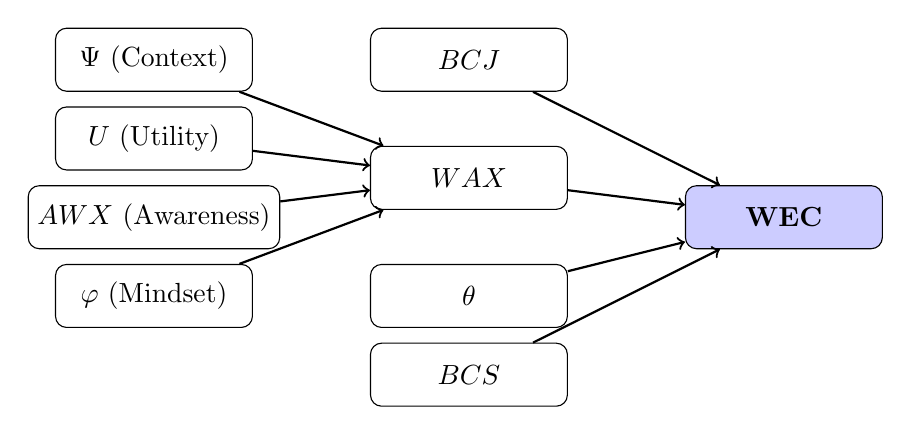
\begin{tikzpicture}[
    box/.style={rectangle, draw, rounded corners, minimum width=2.5cm, minimum height=0.8cm},
    arrow/.style={->, thick}
]
% Inputs
\node[box] (psi) at (0,3) {$\Psi$ (Context)};
\node[box] (u) at (0,2) {$U$ (Utility)};
\node[box] (awx) at (0,1) {$AWX$ (Awareness)};
\node[box] (phi) at (0,0) {$\varphi$ (Mindset)};

% Middle
\node[box] (wax) at (4,1.5) {$WAX$};
\node[box] (theta) at (4,0) {$\theta$};
\node[box] (bcj) at (4,3) {$BCJ$};
\node[box] (bcs) at (4,-1) {$BCS$};

% Output
\node[box, fill=blue!20] (wec) at (8,1) {\textbf{WEC}};

% Arrows
\draw[arrow] (psi) -- (wax);
\draw[arrow] (u) -- (wax);
\draw[arrow] (awx) -- (wax);
\draw[arrow] (phi) -- (wax);
\draw[arrow] (wax) -- (wec);
\draw[arrow] (theta) -- (wec);
\draw[arrow] (bcj) -- (wec);
\draw[arrow] (bcs) -- (wec);
\end{tikzpicture}
\caption{WEC as synthesis of all EBF components}
\label{fig:wec-synthesis}
\end{figure}

%------------------------------------------------------------------------------
\section{Decomposition of WEC}
%------------------------------------------------------------------------------

WEC can be decomposed to identify intervention levers:

\begin{equation}
WEC = \underbrace{\varphi \cdot \min\{U^*\} + (1-\varphi) \cdot \sum U^*}_{WAX} 
    - \underbrace{\theta_{base} + \sum \delta_j \Psi_j}_{\theta}
    \cdot \alpha_{BCJ} \cdot \beta_{BCS}
\end{equation}

where $U^* = AWX \cdot U$ (awareness-modulated utility).

\subsection{Intervention Levers}

To increase WEC, one can:
\begin{enumerate}
    \item \textbf{Increase $\varphi$:} Shift mindset toward complementarity
    \item \textbf{Increase $U$:} Enhance objective benefits
    \item \textbf{Increase $AWX$:} Make benefits salient and concrete
    \item \textbf{Decrease $\theta$:} Lower barriers and friction
    \item \textbf{Advance $BCJ$:} Move person along the journey
    \item \textbf{Target $BCS$:} Design intervention for segment type
\end{enumerate}

%------------------------------------------------------------------------------
\section{Worked Example: Anna's WEC}
%------------------------------------------------------------------------------

\subsection{Baseline}

\begin{align}
WAX &= 0.48 \\
\theta &= 1.32 \\
BCJ &= 3 \text{ (Considering)} \Rightarrow \alpha = 0.6 \\
BCS &= \text{Pragmatische Umweltbewusste} \Rightarrow \beta = 1.0 \\[6pt]
WEC &= (0.48 - 1.32) \cdot 0.6 \cdot 1.0 = -0.50
\end{align}

\textbf{Interpretation:} Negative WEC → very unlikely to act.

\subsection{After Intervention}

\begin{align}
WAX &= 0.90 \\
\theta &= 0.76 \\
BCJ &= 5 \text{ (Acting)} \Rightarrow \alpha = 1.0 \\
BCS &= \text{Pragmatische Umweltbewusste} \Rightarrow \beta = 1.0 \\[6pt]
WEC &= (0.90 - 0.76) \cdot 1.0 \cdot 1.0 = +0.14
\end{align}

\textbf{Interpretation:} Positive WEC → likely to act.

%------------------------------------------------------------------------------
\section{Summary}
%------------------------------------------------------------------------------

WEC is the \textbf{ultimate synthesis} that determines behavioral readiness
in the Moment of Truth. It integrates:
\begin{itemize}
    \item The cognitive dimension ($\varphi$, $AWX$)
    \item The motivational dimension ($U$, $WAX$)
    \item The barrier dimension ($\theta$)
    \item The processual dimension ($BCJ$)
    \item The personal dimension ($BCS$)
\end{itemize}

